\section{Desarrollo Experimental}
El desarrollo del detector de movimiento con sensor infrarrojo PIR (HC-SR501) se llevó a cabo siguiendo una metodología estructurada que incluyó el montaje del circuito, la configuración del sensor y la programación del sistema de control.

\subsection{Materiales}
Para la implementación del proyecto se utilizaron los siguientes componentes:
\begin{itemize}
	\item Raspberry Pi (con 40 pines GPIO)
	\item Placa de expansión GPIO y cable plano
	\item Protoboard
	\item 5 cables puente
	\item Sensor HC-SR501 (sensor PIR)
	\item 1 LED
	\item 1 Resistencia de \SI{220}{\ohm}
\end{itemize}

\subsection{Montaje del Circuito}
El circuito fue ensamblado de acuerdo con el esquema proporcionado en la práctica. La conexión del sensor PIR a la Raspberry Pi se realizó considerando los siguientes aspectos:

\begin{enumerate}
	\item El sensor HC-SR501 se alimentó con 5V desde la Raspberry Pi.
	\item La salida del sensor se conectó al pin GPIO 0 (según la numeración de WiringPi).
	\item El LED indicador se conectó al pin GPIO 1 con una resistencia limitadora de corriente de \SI{220}{\ohm}.
\end{enumerate}

Es importante destacar que el sensor PIR requiere aproximadamente un minuto de inicialización después de ser alimentado, durante el cual puede alternar entre niveles altos y bajos de salida sin relación con la detección de movimiento.

\subsection{Configuración del Sensor}
Previo a la implementación del código, se configuró el sensor PIR ajustando los dos potenciómetros disponibles:

\begin{enumerate}
	\item R1: Se ajustó para establecer el tiempo de retardo de la señal de salida después de detectar movimiento. Para esta práctica, se configuró en un valor intermedio proporcionando un retardo de aproximadamente 5-7 segundos.
	\item R2: Se ajustó para determinar la distancia máxima de detección. Se calibró para detectar movimiento en un rango de aproximadamente 3 metros.
\end{enumerate}

Adicionalmente, se configuró el puente selector en posición "L" para utilizar el modo de disparo no repetitivo, lo que significa que después de detectar movimiento y emitir un nivel alto, el sensor no detectará nuevos movimientos hasta que finalice el tiempo de retardo establecido.

\subsection{Implementación del Software}
El programa para controlar el sistema fue desarrollado en lenguaje C utilizando la biblioteca WiringPi para la interacción con los pines GPIO de la Raspberry Pi. El algoritmo implementado sigue un enfoque simple:

\begin{enumerate}
	\item Configuración de los pines GPIO 0 (sensor) como entrada y GPIO 1 (LED) como salida.
	\item Implementación de un bucle infinito que constantemente verifica el estado del sensor.
	\item Cuando el sensor detecta movimiento, emite un nivel alto que es leído por el programa.
	\item En respuesta a la detección, el LED se enciende y se muestra un mensaje en la terminal.
	\item Cuando no se detecta movimiento, el LED se apaga y se actualiza el mensaje en la terminal.
\end{enumerate}

El código fue compilado y ejecutado utilizando los siguientes comandos:
\begin{verbatim}
	gcc SenseLED.c -o SenseLED -lwiringPi
	sudo ./SenseLED
\end{verbatim}

\section{Resultados}
Los resultados del experimento se documentaron mediante capturas fotográficas que ilustran el funcionamiento del sistema en diferentes situaciones. A continuación, se presentan las imágenes que muestran el comportamiento del detector de movimiento implementado.

\begin{figure}[h]
	\centering
	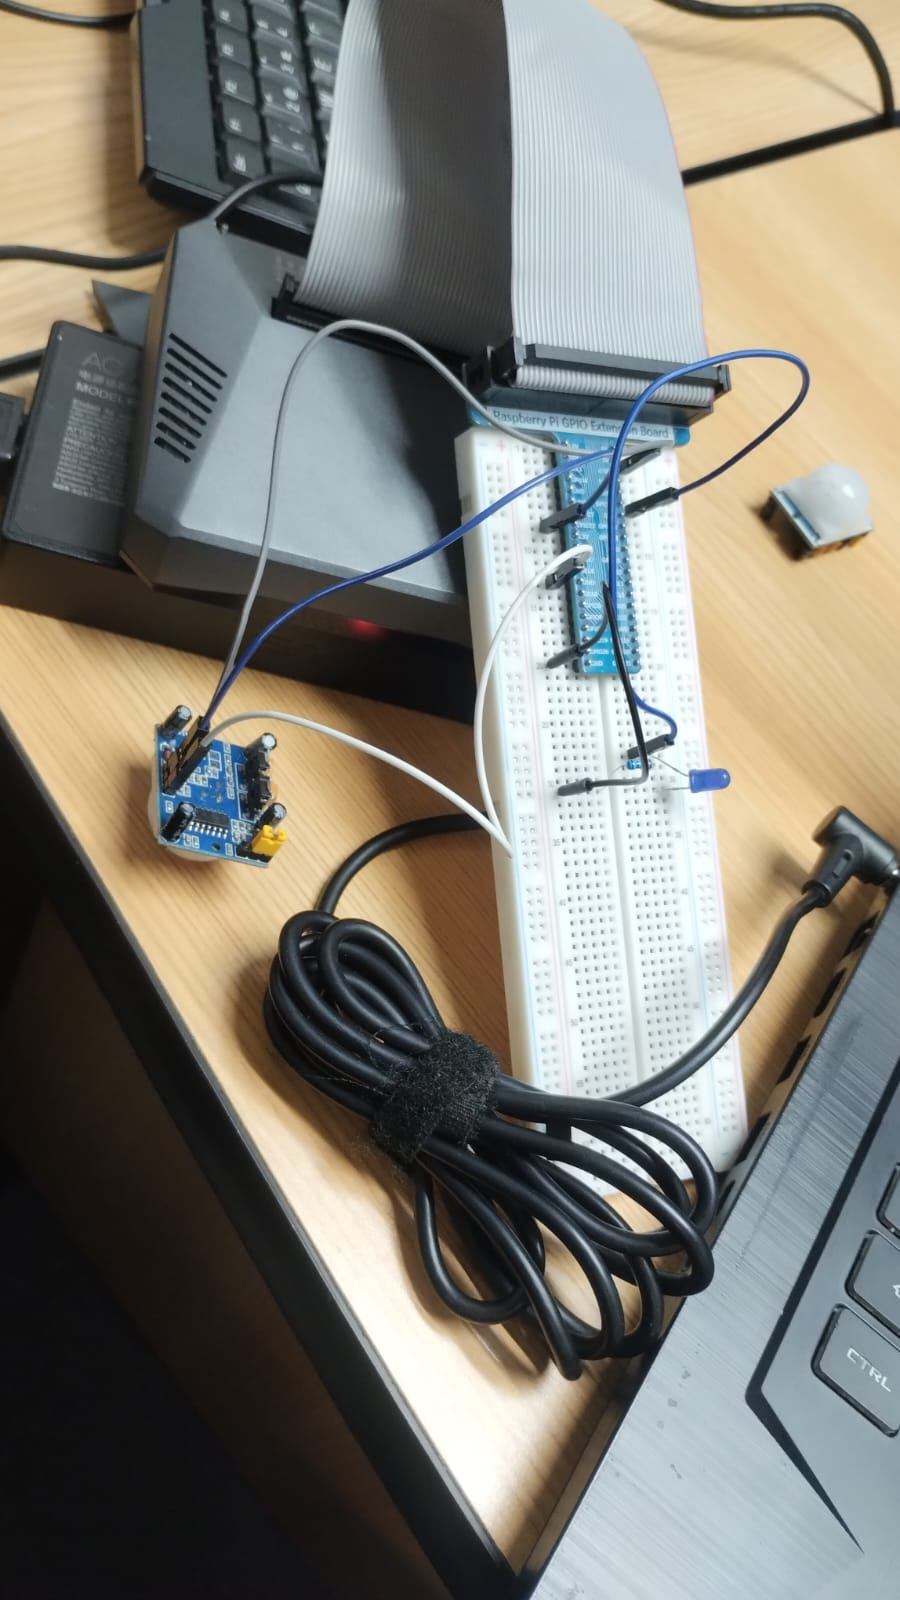
\includegraphics[width=0.5\textheight]{imagenes/1.jpg}
	\caption{Montaje completo del circuito con Raspberry Pi, protoboard, sensor PIR y LED.}
	\label{fig:circuito}
\end{figure}

\begin{figure}[h]
	\centering
	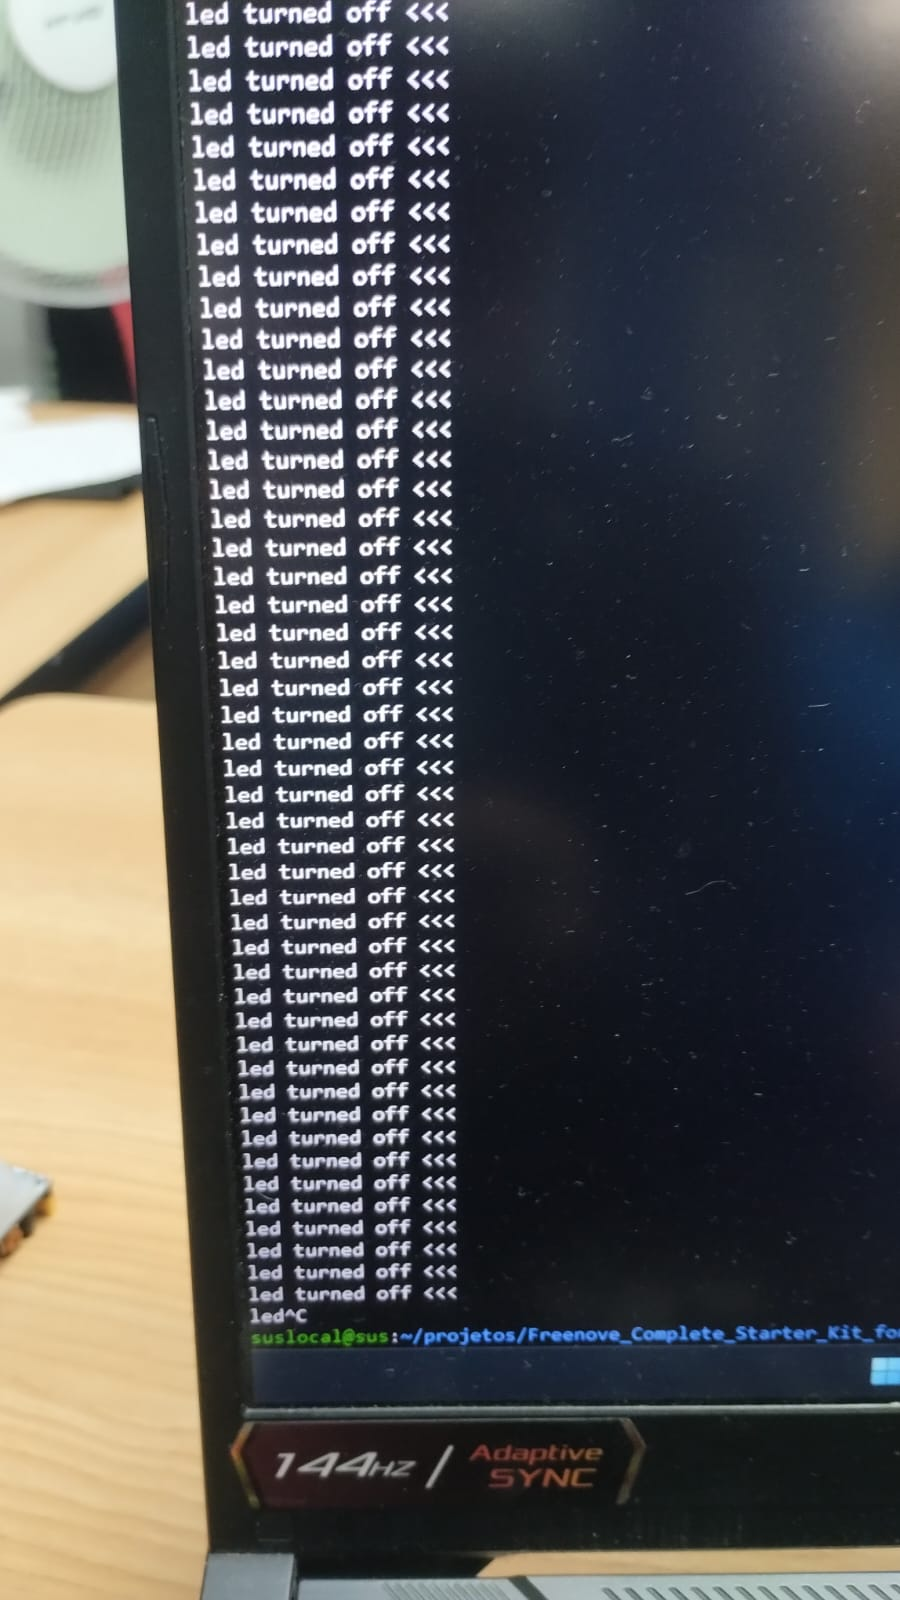
\includegraphics[width=0.5\textheight]{imagenes/2.jpg}
	\caption{Salida en terminal mostrando los mensajes de estado durante la ejecución del programa.}
	\label{fig:terminal}
\end{figure}

\begin{figure}[h]
	\centering
	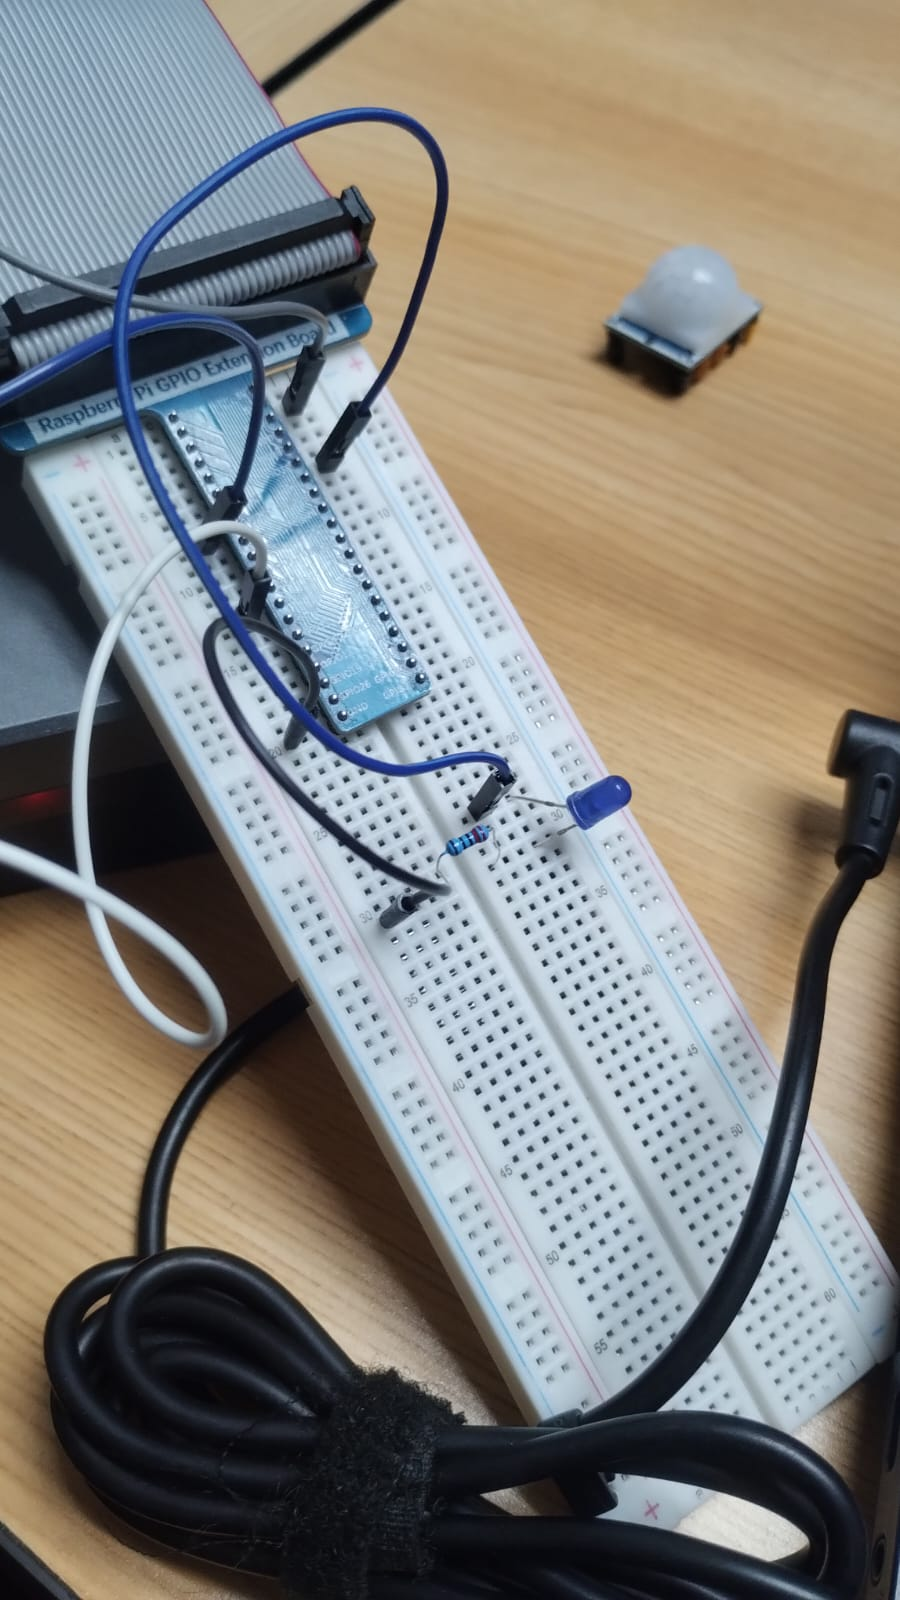
\includegraphics[width=0.5\textheight]{imagenes/3.jpg}
	\caption{Sistema en funcionamiento con LED apagado indicando sin detección de movimiento.}
	\label{fig:deteccionOFF}
\end{figure}

\begin{figure}[h]
	\centering
	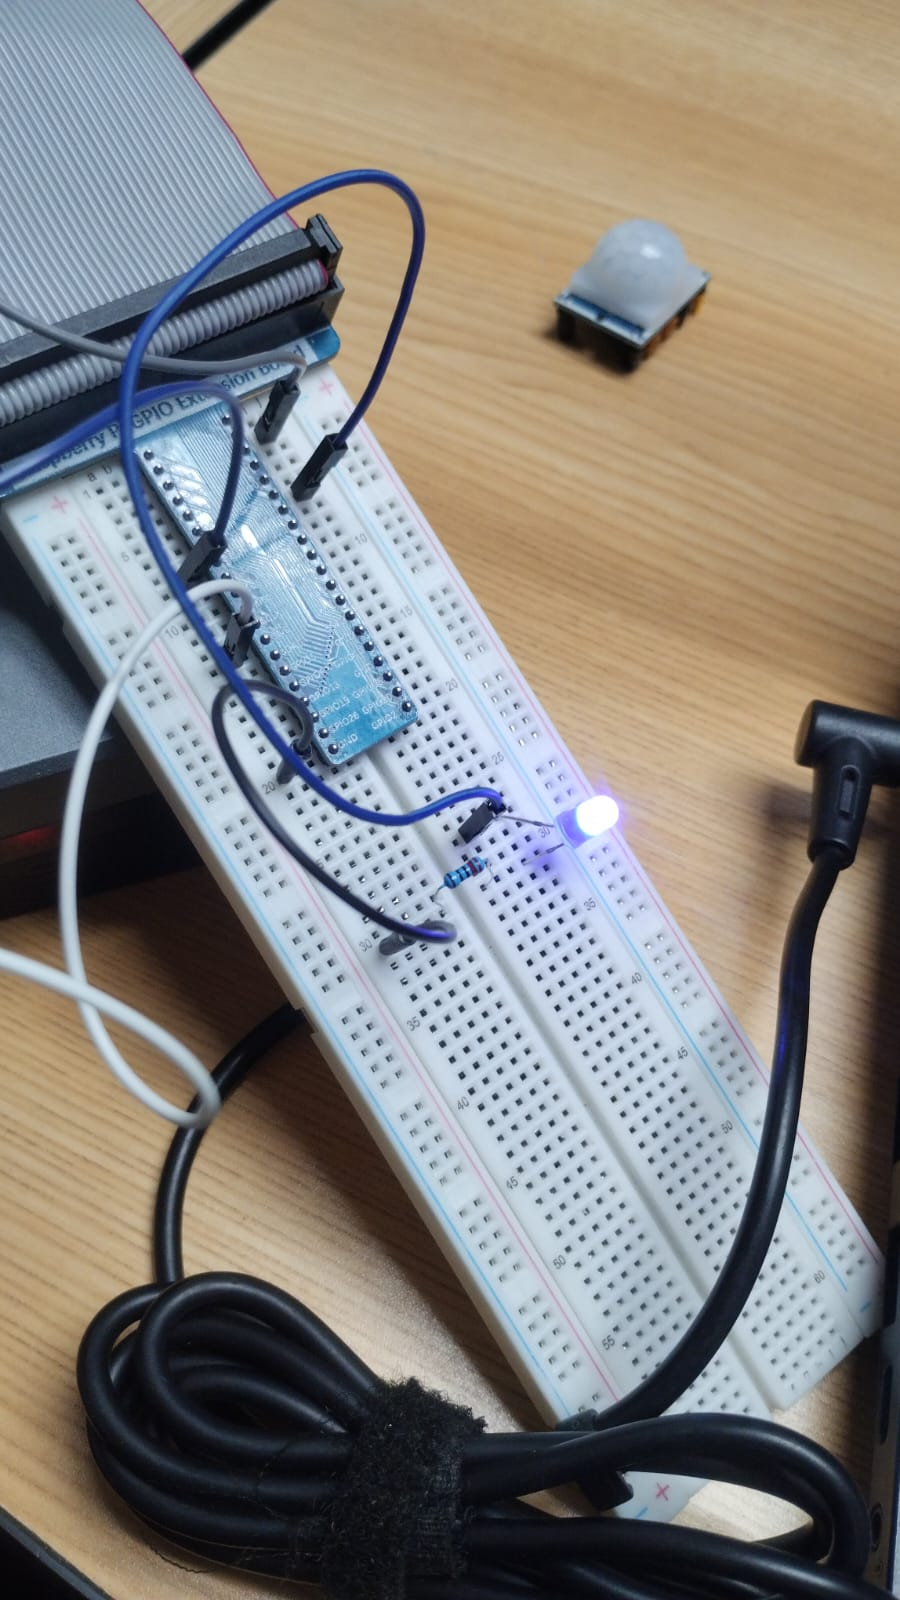
\includegraphics[width=0.5\textheight]{imagenes/4.jpg}
	\caption{Sistema en funcionamiento con LED encendido indicando detección de movimiento.}
	\label{fig:detenccionON}
\end{figure}

Las imágenes ilustran claramente el funcionamiento del sistema de detección de movimiento, mostrando tanto la configuración física como la respuesta del sistema. Se puede observar que el LED se enciende efectivamente cuando se detecta movimiento y se apaga cuando no hay actividad dentro del rango de detección del sensor.